\subsection{Pruebas y resultados}
	Para comprobar la funcionalidad del programa, se realizó la siguiente prueba, se ingresó la cadena ``11''.\\
	Los resultados obtenidos fueron los siguientes:
	
	En la figura \ref{fig:maquin2} se muestra la salida en consola del programa anteriormente ejecutado, en consola se despliega el log de los pasos que va haciendo la máquina así como la cadena que se encuentra actualmente en la cinta, el estado actual y el apuntador.
	\begin{figure}[H]
		\begin{center}
			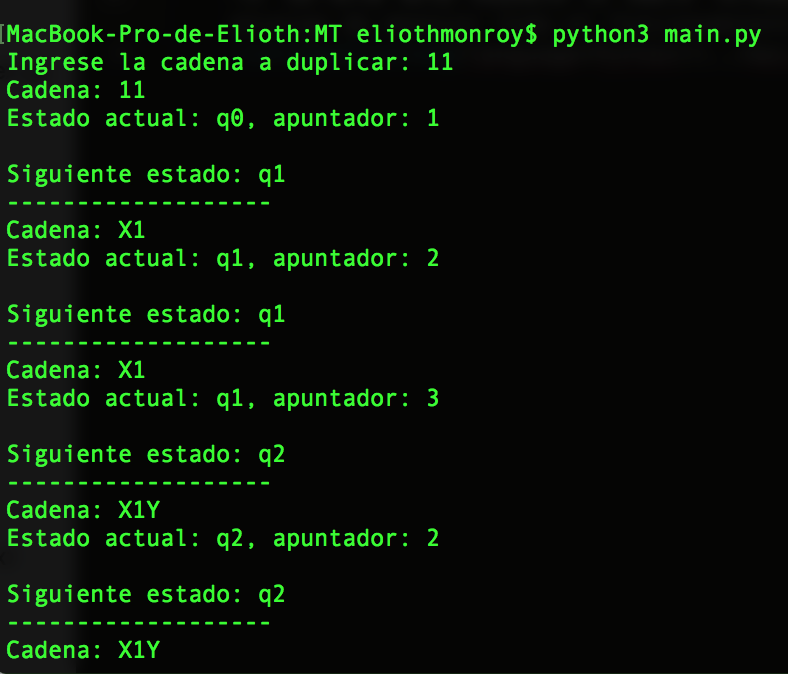
\includegraphics[scale=.8]{MT/img/prueba1.png}
			\caption{Resultados prueba (1)}
			\label{fig:maquin2}
		\end{center}
	\end{figure}

	En la figura \ref{fig:maquin3} se muestra un archivo de log que es generado por el programa al terminar su ejecución, el cual muestra todos los pasos que realizó la máquina, tal y como se mostraron en consola.
	\begin{figure}[H]
		\begin{center}
			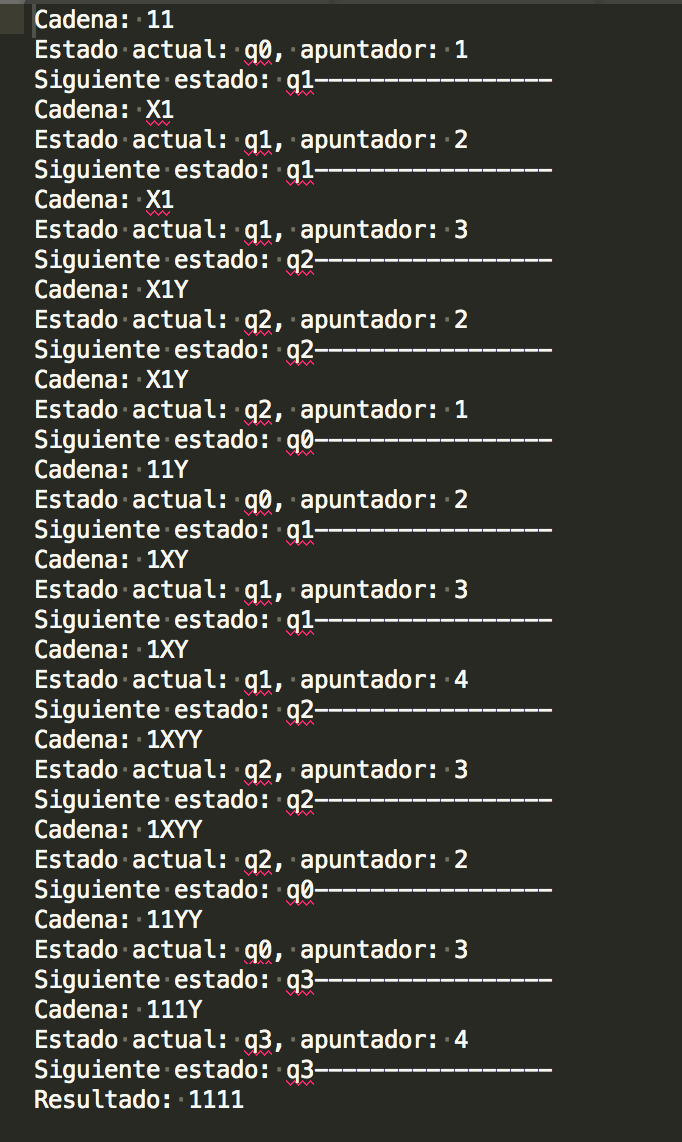
\includegraphics[scale=.8]{MT/img/prueba2.png}
			\caption{Resultados prueba (2)}
			\label{fig:maquin3}
		\end{center}
	\end{figure}
	
	En las figuras \ref{fig:maquin4} y \ref{fig:maquina5} se muestra la ventana del programa en la que se realiza la animación de la máquina de Turing.
	\begin{figure}[H]
		\begin{center}
			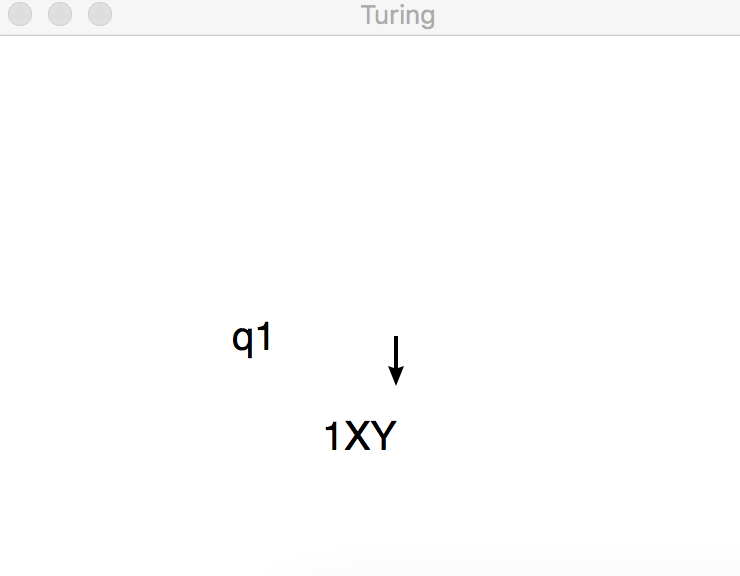
\includegraphics[scale=.7]{MT/img/prueba3.png}
			\caption{Resultados prueba (3)}
			\label{fig:maquin4}
		\end{center}
	\end{figure}
	\begin{figure}[H]
		\begin{center}
			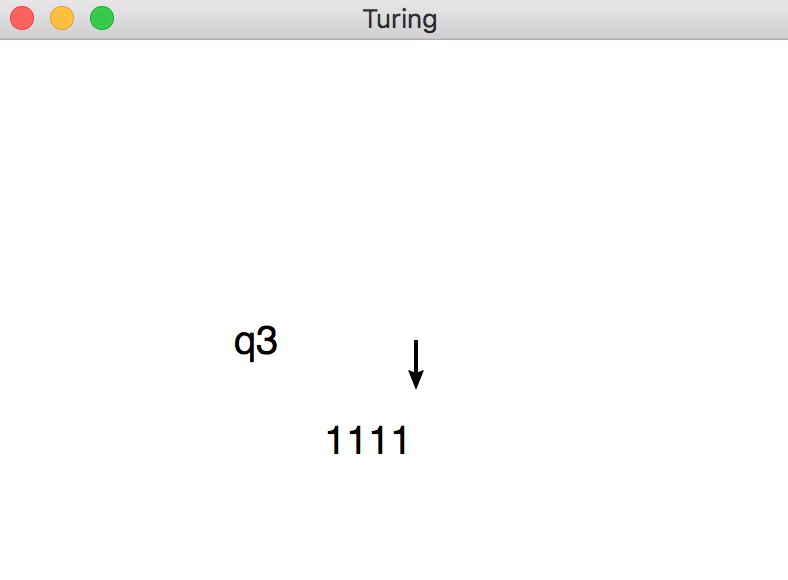
\includegraphics[scale=.7]{MT/img/prueba4.png}
			\caption{Resultados prueba (4)}
			\label{fig:maquina5}
		\end{center}
	\end{figure}

